\documentclass[12pt, a4paper]{report}
\usepackage{amsmath, amssymb, amsfonts}
\usepackage{fancyhdr}
%\setlength{\headheight}{15pt}
\usepackage{geometry}
\geometry{margin=1.5in}
\usepackage[Rejne]{fncychap}
\pagestyle{fancy}
\usepackage{color}
\usepackage{blindtext}
\usepackage{import}
\usepackage{graphicx}
\usepackage{mathrsfs}
\usepackage{trfsigns}
\renewcommand{\chaptername}{Lecture}

\usepackage{import}
\usepackage{listings}
\usepackage{pdfpages}
\usepackage{transparent}
\usepackage{xcolor}

\setlength\parindent{0pt}

\newcommand\ddfrac[2]{\frac{\displaystyle #1}{\displaystyle #2}}

\newcommand{\incfig}[2][1]{%
    \def\svgwidth{#1\columnwidth}
    \import{figures}{#2.pdf_tex}
}

\pdfsuppresswarningpagegroup=1



\title{Systems Dynamics Modeling and Analysis}
\author{Adam Carrera}
\date{January 19, 2021}
\lhead{Week \thepart}

\begin{document}
  \maketitle
  \part{Week 1}
  \chapter{Introduction}

  \section{Syllabus and Textbook}

  Instructor Information:
  \begin{enumerate}
    \item Professor Email: Justin.Koeln@UTDallas.edu
    \item Office hours by appointment
    \item TA Email Sahand.HadizadehKafash@UTdallas.edu
    \item Office hours Friday 1:00 pm - 3:00 and by appointment
  \end{enumerate}

  \noindent
  Textbook: System Dynamics, William Palm 3rd Edition. Chapters 1-9 (not in that order), balance of math, theory, modeling, and application.

  \section{Homework}

  Approximately one assignment per week, due Tuesday before class. No late credit for homework and the lowest score will be dropped. Points will be assigned based on the rubric. Each lecture will have a quiz associated with it, due before the start of next class. The quiz is meant to test your understanding of the material.

  \section{Exam Schedule}

  \begin{itemize}
    \item Exam 1: Week of Thursday, Feb. 25
    \item Exam 2: Week of Thursday, Apr. 8
    \item Final Exam: Week of Monday, May 10
  \end{itemize}

  Open book, open notes exams with a time limit. A calculator is allowed and a formula sheet is provided. Additionally, a sheet of equations that we are expected to know if provided as well.

  \begin{table}
    \centering
    \caption{Grading Criteria}
    \label{tab:table1}
    \begin{tabular}{c c}
      Homework & 30\% \\
      Participation & 10\% \\
      Midterm & 15\% each \\
      Final & 30\%
    \end{tabular}
  \end{table}

  \section{Quiz 1}

  \begin{enumerate}
    \item What year are you in school?
    \item Have you taken systems and controls?
    \item Do you have access to Matlab/Simulink
    \item What is the most important thing you want to remember from this lecture?
    \item What are your goals for the course? ..etc
  \end{enumerate}

  \section{Systems}

  A system is a combination of elements intended to act togehter to accomplish an objective. A systems point of view focuses on how the connections between elements influence overall behavior. We can accept a less-detailed description of individual elements to understand the entire system. We want to look at the general behavior of the system as it evolves over time.

  \begin{figure}
    \centering
    \incfig{subsystems}
    \caption{Subsystem Interaction}
  \end{figure}

  \newpage
  \section{Inputs and Outputs}

  \begin{enumerate}
    \item Input is a cause $ u. $
    \item Output is an effect $ y. $
    \item System dynamics are goverened by input-output relationships $ y = f(t, u). $
  \end{enumerate}

  What is $ y = f(t, u). $ and how can we approximate it?

  \begin{figure}
    \centering
    \incfig{inputoutput}
    \caption{Input-Output Relationship}
  \end{figure}

  \section{Dynamics}

  Mechaincal Engineers study how things behave as a function of location with PDE's.

  \[
      \frac{\partial g(x)}{\partial x} = f(x)
    .\]

  We are more interested in how a system behaves as a function of time, which gives us ODEs $ \frac{dx}{dt} = f(x). $ A static relationship means that the current output only depends on the current input (no dynamics, algebraic relationsship) $ y = f(u(t)). $ A dynamic relationship means that the current output depends on past inputs. Check out 3b1b video on differential equations.

  \[
      \frac{dx}{dt}(t) = f(x(t), u(t)), \quad y(t) = g(x(t))
    .\]

  \section{Modeling}

  A model is a mathematical description of a systems behavior as a function of time. Modeling is to understand the problem, apply simplifying assumptions, and apply appropriate fundamental principles. We need to be able to solve that model for the behavior of that system. This can be done by hand for simple systems. If the model is too complex, a numerical approach may be required. Our goal is to make the model simple enough to work with but realistc enough to trust.

  \newpage

  \subsection{Potato Example}

  We want to be able to heat a potato in 2 minutes with a microwave. We could use a complex model.

  \begin{enumerate}
    \item Capture unique shape
    \item Exact thermal properties
    \item FEA Analysis for temperature distribution
  \end{enumerate}

  We could also use a simple model.

  \begin{enumerate}
    \item Potatoe is a sphere with thermal properties of water
    \item We can solve this problem really quickly using Ch.7
  \end{enumerate}

  The complex model could take days or weeks, but the simple model could take a few minutes. The results could be within 10\% of each other!

  \section{Modeling Ethics}

  We will also discuss modeling ethics. A lot of engineering decisions are made from models. We will focus on understanding the model's limits, what they cannot predict, and what how "simulations are doomed to succeed".








  \chapter{Mathmatical Foundation}

  \section{Objectives}

  \begin{enumerate}
    \item Review Complex numbers
    \item Understand ODEs
    \item Laplace Transforms
  \end{enumerate}

  \section{Complex Numbers}
  $ \sqrt{-1} \equiv i, or j. $ We will use $ j. $ In systems, i is used for current, j is for the complex number. Numbers of the form

  \[
      z = x + iy
    .\]

  are complex numbers in rectangular form. x is the real part, y is the imaginary part. Put the figure of the complex plane here.

  \paragraph{NOTE:} the imaginary part is $ y. $ not $ jy. $

  Some properties of complex numbers are the magnitude and argument.
  \[
      |z| = \sqrt{x ^2 + y ^2}, \quad \theta = \arctan{ \left( \frac{y}{x} \right)}
    .\]

  The complex conjugate is the reflection of a complex number through the real axis.

  \[
      \bar{z} = x = jy
    .\]

  Properties:

  \[
      z + \bar{z} = 2 Re(z)
    .\]

  \subsection{Euler's Formula}

  \[
      e^{j\theta} = \cos{\theta} + j\sin{\theta}
    .\]
  This leads to,

  \begin{align}
    e^{-j\theta} &= \cos{\theta} - j\sin{\theta} \\
    \cos{\theta} &= \frac{e^{j\theta} - e^{j\theta}}{2}
  \end{align}

  \subsection{Polar Form}

  Define magnitude
  \[
      r = |z| = \sqrt{x ^2 + y ^2}
    .\]

  \[
      \theta = \arctan{\frac{y}{x}}
    .\]

    \[
        x = r\cos{\theta}, y = r\sin{\theta}
      .\]

  \subsection{Complex Algebra}

  Addition and subtraction are easily done in rectangular form.

  \[
      z_{1} \pm z_{2} = \left( x_1 + jy_1 \right) \pm \left( x_2 + jy_2 \right)
    .\]

  \noindent
  Multiplication and division are easily done in polar form.


  \subsection{Examples}

  Rectangular to Polar. Remember to think about quadrants!

  \begin{align}
    z &= 1 - j \\
    |z| &= \sqrt{1 ^2 + (-1 ^2)} \\
    \theta &= \arctan{\frac{-1}{1}} = 45^{\circ}
    z &= \sqrt{2} e^{-j \frac{\pi}{4}}
  \end{align}

  Division, can be done in rectangular form by multiplying by the complex conjugate. Can also be done in polar form.

  \begin{align}
    \frac{3 + 2j}{1 - 3j} &= \frac{3 + 2j}{1 - 3j} * \frac{3 + 2j}{1 + 3j} \\
    \frac{3 - 6 + 2j + 9j}{1 + 9} &= \frac{-3 + 11j}{10}
  \end{align}

  Powers, $ z = 1 - j, z ^2 = ?. $
  \begin{align}
    z &= \sqrt{2}e^{-j \frac{\pi}{4}} \\
  \end{align}

  In fact,

  \[
      z^n = re^{j\theta}n = r^n e^{jn\theta}
    .\]

  \subsection{Complex Functions}

  \[
      z_1 \rightarrow G(z_1) \rightarrow z_2
    .\]

  Example,

  \[
      G(z_1) = \frac{z_1 + 2}{z_1^2 + z_1 + 1}
    .\]

  let $z_1 = j2$. We can evaulate the function by plugging in $ j2. $ for $ z_1. $

  \section{ODEs - Basics}

  Independent variable is time, $ t. $ The dependent variable is usually denoted as $ x. $

  Derivatives,

  \[
      \dot{x} = \frac{dx}{dt}, \quad \ddot{x} = \frac{d^2 x}{dt^2},  \quad \ldots \quad x^{(n)} = \frac{d^n x}{dt^n}
    .\]

    Standard form is to have all functions of the dependent variable on the LHS, all isolated constants and functions of time on the RHS. The RHS is considered the input or the forcing function. If the RHS = 0 the equation is homogeneous. If not, it is nonhomogeneous.

    The goal is to solve for $ x(t). $ This gives us the solution or the response.

    \subsection{Examples of Standard Form}

    \begin{align}
      \ddot x + 3 \dot x + 5x &= 0 \\
      \ddot x + 3\dot x x +5 x ^2 &= 5 \sin{2t} \\
      \dot x &= 6 + 5 \sin t
    \end{align}

    \subsection{Initial COnditions}


    When solving an ODE, there is a family of solutions. Example:

    \[
        2 \dot x + 6x = 3 \quad x(t) = Ce^{-3t} + 0.5
      .\]
    you could choose many values for C and still have a solution to the equation. No matter the value of C, $ x(t). $ still approaches 0.5. Include the graph here. Without loss of generality, we assume that the system starts at $ t = 0. $ Determining C requires knowledge of x at some time t. Commonly, the initial condition is given as $ x(t_0) = x_0. $

    \subsection{Classification of ODEs}

    Linearity generally means that $ f(x + y) = f(x) + f(y). $ Linear ODEs contain only linear functions of the dependent variable and its derivatives. Nonlinear functions of the independent variable do not make an ODE nonlinear.

    The order is the highest derivative of the dependent variable (double dot, 2nd order). A coupled set of ODEs can be reducded to a single ODE whose order is the sum of the oder of the individual ODEs.

    Example:

    \begin{align}
      3 \dot{x_1} + 5 \dot{x_2} - 7 x_2 &= 5 \\
      \dot x_2 + 4 x_1 + 6 x_2 &= 0
    \end{align}

    Add the sum of the orders of the two dependent variables. 1 order from x1 and 1 order from x2. This is a second order system, which could be represented by a single 2nd order ODE.

    \subsection{Combining Coupled ODEs}
    We have two equations.
    \begin{align}
      \dot x_1 + 4x_2 &= 3 \\
      2 \dot x_2 + x_1 &= 5
    \end{align}

    Solution,

    \[
        \dot x_1 + 4x_2 = 3 \Rightarrow \ddot x_1 + 4 x_2 = 0
      .\]

    Rearrange the second equation for x2 and substitute.

    \section{Solution}

    \subsection{Direct Integration}

    With some first order ODEs, we can rearrange as

    \[
        \frac{dx}{dt} = f(t)
      .\]
    and integrate both sides.

    \[
        \int{dx} = \int{f(t) dt}
      .\]

    \[
        x(t) = x(t_0) + \int{f(t)dt}
      .\]

    Example $ \dot x = 5. $

    \subsection{Seperation of Variables}
    Doesn't show up that often in this class.
    \[
        \frac{dx}{dt} = g(t) f(t)
      .\]

    \subsection{Trial-Solution Method}

    For any nth order linear ODE, there is a response $ x(t) = x_h + x_p. $ The response is the sum of the homogeneous solution and the particular solution. The sum of the internal behavior and the external behavior.

    Assume the solution is of the form $ x(t) = e^{\lambda t}. $ Take the derivative of $ x(t). $ n times and substitute into the ODE. Note that $ e^{\lambda t} \neq 0. $ This gives us the characteristic equation.

    \[
        (\lambda - \lambda_1)( \ldots ) = 0
      .\]




  \part{Week 2}

  \chapter{ODEs and Laplace Transforms}

  \section{Trial Solution}

  \subsection{Characteristic Equation}
  Plug in the form of the solution
  \[
      x(t) = e^{\lambda t}
    .\]
  \subsection{Example}
  \begin{align}
    \ddot x + 10 \dot x + 9x &= 5 \sin 2t \\
    \ddot x + 10 \dot x + 9x &= 0 \\
    \lambda ^2 + 10 \lambda + 9 &= 0 \\
    (\lambda + 9)(\lambda + 1) &= 0
  \end{align}

  The roots are distinct. -9, -1. The roots can be repeated, or complex as well!

  \subsection{Types of Roots}
  If all roots are distinct, there will be n different coefficients.

  \[
      \dot x + ax = 0, \quad x(t_0 = 0) = 0
    .\]
  \[
      (\lambda + a) e^{\lambda t} = 0, \quad \lambda = -a
    .\]

  \[
      x_0 = C e^{-a*0} = C, \quad x(t) = x_0 e^{-at}
    .\]
  If we have repeated roots, the coefficients gain increasing powers of time.

  \[
      x(t) = C_1 e^{\lambda t} + C_2 t e^{\lambda t} \ldots
    .\]

  Complex roots can be handled using Euler's formula.

  \[
      \lambda_{i, i+1} = \sigma \pm j\omega
    .\]

  \[
      x(t) = \ldots + C_i e^{\sigma + j\omega} + C_{i + 1} e^{\sigma - j\omega} + \ldots
    .\]
  Using eulers formula,

  \[
      x(t) = \ldots + \left( C'_i \cos \omega t + C'_{i+1} \sin \omega t \right) e^{\sigma t} + \ldots
    .\]
  The prime means that the coefficient is different from the line above. This solution is going to be oscillating.

  \section{Forced Response}

  Just discussed how to obtain $ x_h. $ Use Method of Undetermined Coefficients to get $ x_p. $ Choose a solution form based on the term in $ f(t). $

  \begin{table}
    \caption{Solution Forms}
    \centering
    \begin{tabular}{c  c}
      Term in $ f(t). $ & Form of solution $ x_p(t). $ \\
      $ A_n^t + \ldots + A_1 t + A_0. $  & $ C_n^t + \ldots + C_1 t + C_0. $\\
      $ Ae^{at}. $ & $ Ce^{at}. $ \\
      $ A\sin \omega t$ & $ C\sin \omega t . $ \\
      $ Ae^{at}\sin \omega t. $ & $ Ce^{at}\sin \omega t. $
    \end{tabular}
    \label{tab:forcedresponse}

  \end{table}
  Note, the form of the forcing function always shows up i nthe form of the solution (property of linear ODEs) See Table \ref{tab:forcedresponse}

  Substitute assumed forms of $ x_p. $ int othe ODe and determine the coefficients, then go back and solve the homogeneous problem seperately. Add the two solutions with linear superpositions. Finally, find the coefficients to the homogeneous solution.


  \newpage

  \section{Laplace Transforms}
  Finding solutions in the time domain is hard. While using laplace transforms takes longer, the solution is generally easier to find (algebra over calculus). The laplace transform is a linear operator, so it is useful for

  \begin{enumerate}
    \item Nonhomogeneous equations with a forcing function of time
    \item Sets/systems of equations
  \end{enumerate}

  Linear ODEs become algebraic relationships, and convolution becomes multiplication.

  \begin{equation}
    F(s) = \mathcal{L}\{f(t)\} = \int_{0-}^{\infty} e^{st} f(t)dt
  \end{equation}

  Assume $ f(t) = 0, t < 0. $ We tend to start caring about what happens at time $ t = 0. $ However, interesting "stuff" happens at time $ t = 0. $

  \begin{enumerate}
    \item "stuff" - step changes, impulses
    \item We need a way to denote before and after this stuff happens
  \end{enumerate}

  Let $ \epsilon, $ be an infitessimally small unit of time. $ 0-, 0+ $ occur $ \epsilon $ seconds before and after time $ t = 0. $ Unless stated explicitly, we assume $ f(t) = 0 \forall t < 0. $

  \subsection{Inverse Laplace Transform}

  The definition of inverse laplace tranforms is complex, so we use lookup tables in the book.

  Some common examples,

  \[
      f(t) = e^{-at} \iff F(s) = \frac{1}{s + a}, \quad a > 0
    .\]

  \subsection{Properties}

  Laplace Transforms are linear. Inverse Laplace transforms too.

  \[
      \mathcal{L}\{af(t) + bg(t)\} = a \mathcal{L}\{f(t)\} + b \mathcal{L}\{g(t)\}
    .\]

  This property does NOT hold for multiplication. Instead, multiplication corresponds to a convolution integral in the time domain.

  \[
      F(s)G(s) = \mathcal{L}\left\{\int_0^t f(t)g(t - \tau) d\tau\right\}
    .\]

  Derivatives,

  \begin{equation}
    \mathcal{L}\{\dot{f(t)}\} = sF(s) - f(0)
  \end{equation}

  \begin{equation}
    \mathcal{L}\{\ddot{f(t)}\} = s ^2 F(s) - sf(0) - \dot{f(0)}
  \end{equation}

  Integrals,

  \[
      \mathcal{L}\left\{\int f(\tau)d \tau \right\} = \frac{1}{s} F(s)
    .\]


  \chapter{Laplace Transforms}

  \section{Laplace Transforms of Special Functions}

  \begin{enumerate}
    \item Unit Step $ \mathcal{L}\{u_s\} = \frac{1}{s}. $
    \item Unit Ramp $ \mathcal{L}\{u_r\} = \frac{1}{s ^2}. $
    \item Unit Pulse $ \mathcal{L}\{u_p\} = \frac{1}{sD} \left( 1-e^{sD} \right). $
    \item As D approaches zero, we get the unit impulse function
    \item $ \mathcal{L}\{\delta(t)\} = 1. $
  \end{enumerate}

  \section{Properties of Laplace Transforms}

  \subsection{Time Shift}
  Many time shifts occur due to distance traveled. E.g. Flow through a pipe. A time shift results in a multiplication by an exponential in the frequency domain.
  \[
      \mathcal{L}\{f(t-\alpha)\} = e^{-\alpha s}F(s)
    .\]

  \subsection{Multiplication by Exponential}
  Multiplication by an exp in the time domain results in a shift in the frequency domain.
  \[
      \mathcal{L}\{e^{-\alpha t}f(t)\} = F(s + \alpha)
    .\]

  \section{Initial Value Theorem}

  Sometimes we would like to find the value of $ x(t) $ at $ t = 0^+. $ Given the laplace transform of the function we have the initial value theorem (IVT)

  \begin{equation}
    x(0^+) = \lim_{t \rightarrow 0} x(t) = \lim_{s \rightarrow \infty} sX(s)
  \end{equation}

  This is only applicable if the limit exists, and the transforms and derivatives of $ x(t) $ exist.

  \section{Final Value Theorem}

  Sometimes we would like to know the limit of a function as time goes to infinity. If the limit exists, and transforms/derivatives of $ x(t) $ exist we have the final value theorem (FVT).

  \begin{equation}
    \lim_{t \rightarrow \infty} x(t) = \lim_{s \rightarrow 0} sX(s)
  \end{equation}

  \section{Example - Solving ODE with Laplace}

  We have the EOM,

  \[
      m\ddot x + c \dot x + kx = 0
    .\]
  \noindent
  laplace transform and initial conditions gives us

  \[
      m(s ^2X(s) -s) + c(sX(s) - 1) + kX(s) = 0
    .\]
  \noindent
  rearrange,
  \[
      (ms ^2 + cs + k)X(s) = ms + c
    .\]

  \[
      X(s) = \frac{ms + c}{ms ^2 + cs + k}
    .\]

  \subsection{Partial Fraction Expansion}
  we can find $ x(t) $ with inverse laplace transforms. Our transfer function is a ration of polynomials.

  \[
      X(s) = \frac{N(s)}{D(s)}
    .\]

  \noindent

  Our goal is to express $ X(s)$ as a suitable sum of fractions by dividing $ D(s) $ into 1st and 2nd order roots. Then we can preform the inverse laplace transform.

  \subsubsection{Case 1: Distinct Roots}

  If $ D(s) $ contains $ (s + p_i). $ The corresponding factor is,

  \[
      \frac{A_i}{s + p_i}
    .\]

  where $ A_i $ is the called the "residue".

  \subsubsection{Case 2: Repeated Roots}

  If $ D(s) $ contains $ (s + p_i)^{r_i}. $ The corresponding factor is,

  \[
      \frac{A_{r_i}}{ \left( s + p_i \right)^{r_i} } + \frac{A_{r_i-1}}{ \left( s + p_i \right)^{r_{i}-1} } + \ldots
    \]

  from the table,

  \begin{equation}
    \mathcal{L}^{-1}\left\{\frac{1}{(s+a)^n}\right\} = \frac{1}{(n-1)!}t^{n-1}e^{-at}
  \end{equation}

  increase the power of t as you have more repetition!

  \subsubsection{Case 3: Complex Roots}

  If $ D(s) $ contains $ s ^2 + as + b. $ The corresponding factor is,

  \[
      \frac{Bs + C}{s ^2 + as + b}
    .\]

  Before taking the inverse Laplace transform, we need to complete the square

  \[
      s ^2 + as + b = (s + \sigma) ^2 + \omega ^2
    .\]

  eg,

  \[
      s ^2 + 2s + 2 = (s ^2 + 2s + 1) + 1 = (s + 1) ^2 + 1
    .\]

  The goal is to write in terms of sine and cosine. This introduces oscillation in our signal.

  \[
      = A_1 \mathcal{L}^{-1}\left\{\frac{s + \sigma}{(s + \sigma) ^2 + \omega ^2}\right\} + A_2 \mathcal{L}^{-1}\left\{\frac{\omega}{(s + \sigma) ^2 + \omega ^2}\right\}
    .\]

  \section{Parts of the Response}

  The \textbf{Transient Reponse} is the part that disappears with time. The parts that remain with time are the \textbf{Steady-state Response}. The \textbf{Free Response} is the part that depends on the ICs, and the \textbf{Forced Response} is the part due to the forcing function. We can write the total response as a sum of the transient and steady state or the sum of the free and forced response! Note that we will not always have two terms.

  \section{Transfer Functions}

  \textbf{Transfer Functions} capture the dynamics of the system \textbf{independent of ICs and input} (forcing functions)

  \begin{equation}
    T(s) = \frac{X(s)}{F(s)}
  \end{equation}

  example,

  \[
      \dot x + ax = f(t) \Rightarrow (s+a)X(s) = F(s)
    .\]

  \[
      T(s) = \frac{X(s)}{F(s)} = \frac{1}{s+a}
    .\]

  Denominator of transfer function is the caracteristic equation, it can tell us about the general behavior of the system.

  \[
      T(S) = \frac{1}{s ^2 + 7s + 10}, \quad r = -2, -5
    .\]

  \begin{itemize}
    \item Roots are real - no oscillation in response
    \item Roots are negative - model is stable and free response converges to zero
  \end{itemize}



  Transfer function is internal to the system, and is a mapping between the input and the output. We can also go back and forth between ODE and Transfer Function.

  \[
      G: X \rightarrow F
    .\]

  The transfer function is a ratio of polynomials. The system zeroes are the roots of the numerator and the poles are the roots of the denominator.

  Example,

  \[
      G(s) = \frac{s + 1}{s + 2}
    .\]

  has a zero at -1 and a pole at -2. Zeroes are given by models with derivatives of the input. The numerator dynamics can significantly alter the response but the analysis is the same.

  Note,

  \[
      g(t) = u_s(t) \Rightarrow \dot g(t) = \delta (t)
    .\]

  \section{Transfer Function and Convolution}

  For LTI systems, teh system response is the convolution of the input function and the system's impulse response. From the definition of a transfer function, the response of our system is,

  \begin{equation}
    X(s) = G(s)F(s)
  \end{equation}

  We can also think about $ G(s) $ as the impulse response of our system.

  \[
      f(t) = \delta (t) \Rightarrow F(s) = 1 \Rightarrow X(s) = G(s)F(s) = G(s) \cdot 1
    .\]



  \section{section name}

  \part{Week 3}

  \chapter{Transfer Functions}

  \section{Quiz Review}
  \begin{itemize}
    \item L4Q3 - Remember that the transfer function is independent of initial conditions!
  \end{itemize}

  \section{Value of Transfer Functions}

  Transfer functions are useful when working with matlab and simulink. They are the basis for block diagrams. Simulink is how you program block diagrams. Transfer functions can scale with multiple inputs and outputs as well. We can determine a transfer function for each IO pair.

  \[
      T_{ab}(S) = \frac{X_a(S)}{U_b(S)}
    .\]

  \subsection{Multiple Input Eample}
  We can derivate a transfer function for each input by temporarily assuming all other inputs are zero.
  \[
      5 \ddot x + 30 \dot x + 40x = 6f(t) - 20g(t)
    .\]

  \begin{align*}
    T_1(S) &= \frac{X(S)}{F(S)} = \frac{6}{5s ^2 + 30s + 40} \\
    T_2(S) &= \frac{X(S)}{G(S)} = \frac{-20}{5s ^2 + 30s + 40}
  \end{align*}

  Note that the denominators are the same. By \textbf{superposition}, the total response is,

  \[
      X(S) = T_1(S)F(S) + T_2(S)G(S)
    .\]

  \subsection{Multiple Ouputs}

  Systems of equations may have more than one dependent variable. We can derive transfer functions for each as well.

  Example:
  \begin{align*}
    \dot x &= -3x + 2y \\
    \dot y &= -9y -4x + 3v(t)
  \end{align*}
  Transform Equations:
  \begin{align*}
    sX(s) &= -3X(s) +2Y(s) \\
    sY(S) &= -9Y(s) - 4X(S) + 3V(S) \\
  \end{align*}
  Eliminate all variables except for desired output and input.
  \[
      X(S) = \frac{2}{s+3}Y(S), \quad Y(S) = \frac{1}{s+9} \left( -4X(s) + 3V(s) \right)
    .\]

  \[
      X(S) = \frac{2}{s+3} \left( \frac{1}{s+9} (-4X(S) +3V(s)) \right)
    .\]

  \[
      \frac{X(s)}{V(S)} = \frac{6}{s ^2 + 12s + 35}
    .\]

  \[
      \frac{Y(S)}{V(S)} = \frac{3(s+3)}{s ^2 + 12s + 35}
    .\]

  Note again that they have the same denominator! That is because the two equations represent one system.

  \subsection{Fluid Tank}

  For one tank, we will learn how to derive,

  \[
      \frac{Q_{out}(S)}{Q_{in}(S)} = \frac{1}{RCs + 1}
    .\]

  What if we had two tanks?

  \[
      \frac{Q_{12}(s)}{Q_{in}(s)} = \frac{1}{R_1C_1s + 1}
    .\]

    \[
        \frac{Q_{out}(s)}{Q_{12}(s)} = \frac{1}{R_2C_2s + 1}
      .\]

  \[
      \frac{Q_{out}(s)}{Q_{in}(s)} = \frac{Q_{out}(s)Q_{12}(s)}{Q_{12}(s)Q_{in}(s)}
    .\]

    \textbf{SLIDE 13}

  \section{Block Diagrams}

  Can use transfer functions of a system/model to construct a visual representation of the dynamics - \textbf{Block Diagram}. They show the physical connections of the system, and the cause and effect relationships between components. Block diagrams can be directly used to develop simulation diagrams in Simulink.

  \subsection{Basic Symbols}

  \begin{itemize}
    \item Arrow - represents a variable/signal with direction showing cause and effect relationship. Can be labeled with the signal name in the laplace domain.
    \item Block - input-output relation of a transfer function.
    \item Circle (summation) - Addition or subtraction of signals.
    \item Takeoff point - obtain value of variable for use elsewhere. Note that you cannot branch a signal into another.
    \item Multiplier (Gain) $ X(s) = KF(s). $
    \item Integration  $ X(s) = \frac{1}{s}F(s) = x(t) = \int f(t)dt. $ This is used to represent $ \dot x = f(t). $
  \end{itemize}

  \subsection{Equivalent Block Diagrams}

  \begin{itemize}
    \item Block diagrams are not unique
    \item More than one diagram can represent the same model
  \end{itemize}
  Example:
  \[
      \dot x + 7x = f(t) \Rightarrow \frac{X(s)}{F(s)} = \frac{1}{s+7}
    .\]

  Can also be written as,

  \[
      X(s) = \frac{1}{s} \left( F(s) - 7X(s) \right)
    .\]

  The above equation can be written with a transfer function block, and the below equation can be written with a negative feedback loop.

  \subsection{Block Algebra}

  Blocks in series can be multiplied. For blocks $ T_1, \ldots T_n. $ in series,

  \[
      X(s) = \prod_{n=1}^{k} T_n
    .\]

  Blocks in parallel are added together. For blocks $ T_1, \ldots T_n. $ in parallel,

  \[
      X(s) = \sum_{n=1}^{k} T_n
    .\]

  \textbf{Add in the closed loop feedback}






  \chapter{Block Diagrams}

  \section{Block Diagram from System Model}

  \[
      3 \dot y + y = 2u
    .\]

  Take laplace transform and arrange highest power of $ s $ on the left.

  \begin{align}
    3sY(s) + Y(s) &= 2U(s) \\
    sY(s) &= \frac{1}{3} \left( 2U(s) - Y(s) \right)
  \end{align}

  \begin{itemize}
    \item Draw output signal going to the right
    \item Draw string of integrators
    \begin{itemize}
      \item \# of integrators = highest power of $ s $
      \item In this case just 1 integrator
    \end{itemize}
    \item Draw a gain block corresponding to the common coefficient on the RHS
    \item Add summation block
    \item Use existing signals to build up the sum of terms on the RHS
  \end{itemize}

  \begin{figure}
    \centering
    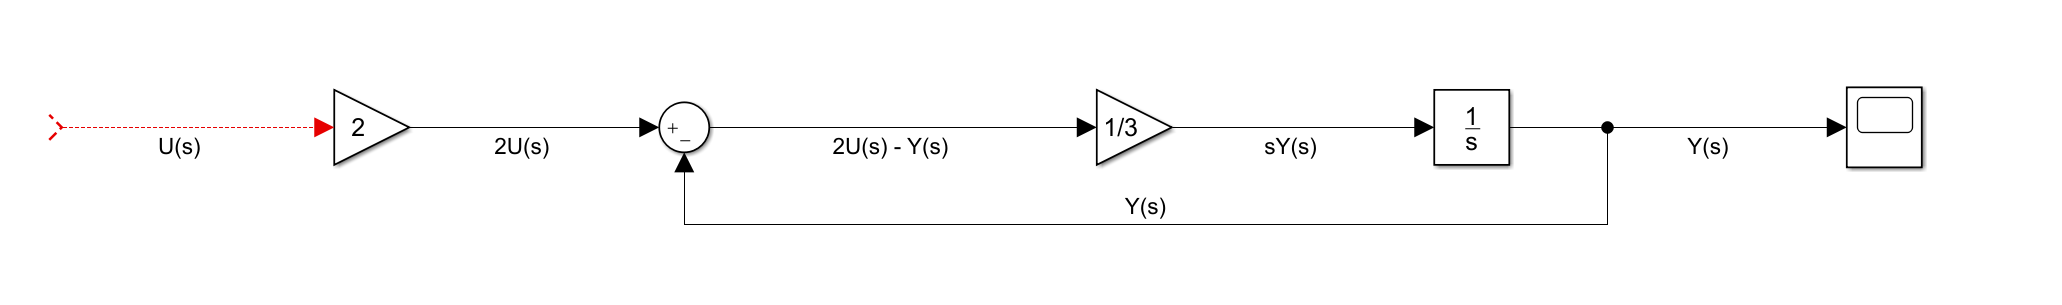
\includegraphics[width=\textwidth]{figures/blockdiagram1}
    \caption{Example Block Diagram}
  \end{figure}

  \begin{figure}
    \centering
    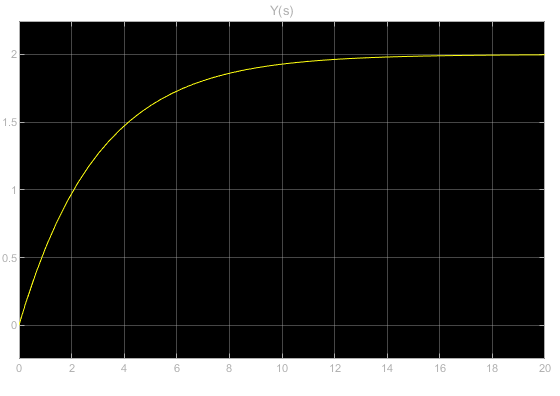
\includegraphics[width=0.8\textwidth]{figures/scope1}
    \caption{Scope output of 6.1}
  \end{figure}

  \subsection{Alternative Approach}

  This can be done in the time domain as well.

  \[
      \ddot x + 2\dot x + 3x = f(t)
    .\]

  Isolate highest derivative,

  \[
      \ddot x = f(t) - 2\dot x - 3x
    .\]

  String integrators to get x, and add terms to compute the highest derivative.

  \section{Transfer Function and the IO equation}

  Can go backwards from tansfer function to ODE.

  \[
      G(s) = \frac{s + 1}{s ^2 + 3s + 5}
    .\]

  \[
      (s ^2 + 3s + 5) Y(s) = (s + 1) U(s)
    .\]

  \[
      \ddot y + 3 \dot y + 5y = \dot u + u
    .\]

  \section{Transfer Function to State-Space}

  For MIMO systems, we have see that the transfer function looks like

  \begin{equation}
    Y(s) = G(s)U(s)
  \end{equation}

  Where Y, G, and U are matricies. Each transfer function in G has the same denominator. However, this is not always the most convient representation of the system. \textbf{State-space form} is the transform of system of ODEs of various orders into a larger system of 1st order ODEs.

  \subsection{State Variables}

  State variables form the smallest set of independent variables that completely describe the state of a system. If you know the initial values and input trajectories you can predict the state/output trajectories for the system. \textbf{State variables are independent}, and cannot be expressed as algebraic functions of another and the system inputs. Additionally, \textbf{State variables are not unique} and the number of state variables is equal to the number of initial conditions.

  \subsubsection{Example: Mass-Spring-Damper}

  Given MSD system with $ m = 1, k = 2, c = 1. $

  \[
      \ddot x + \dot x + 2x = f(t), \Rightarrow \frac{X(s)}{F(s)} = \frac{1}{s ^2 + s + 2}
    .\]

  This is a second order system, so we need two initial conditions. But what are the states?

  \begin{enumerate}
    \item Position $ x_1 = x. $
    \item Velocity $ x_2 = \dot x. $
  \end{enumerate}

  Initial conditions are only needed for state variables $ x(0) \dot x(0). $

  \subsection{State-Variable Equations}

  There are as many state-variable equations as there are state variables. Each state-variable equation is a \textbf{1st order ODE}.

  \begin{enumerate}
    \item Left side - derivative of a state variable
    \item Right side - only a function of state variables, system inputs, maybe time $ t. $
  \end{enumerate}

  General form,

  \begin{equation}
    \dot x_i = f_i(x_1, \ldots, x_n, u_1, \ldots, u_n)
  \end{equation}

  \subsubsection{Example Cont}

  The original ODE can be rearrange in terms of the state variables,

  \[
      \ddot x + \dot x + 2x = f(t) \Rightarrow \dot x_2 + x_2 + 2x_1 = f(t)
    .\]

  Where,

  \[
      x_1 = x, x_2 = \dot x \Rightarrow \dot x_1 = x_2, \dot x_2 = \ddot x
    .\]
  This gives us,
  \[
      \dot x_2 = -2x_1 - x_2 + f(t), \dot x_1 = x_2
    .\]

  \section{State equation - Nonlinear}

  In general, the nonlinear state space form is,

  \section{State Equation - Linear}

  If all elements are linear, then the state vector are a linear combination of the states.

  \begin{equation}
    \dot x = Ax + Bu
  \end{equation}

  where,

  \begin{itemize}
    \item State vector $ \dot x. $
    \item Dynamics matrix $ A. $
  \end{itemize}

  \subsection{Output Equation}

  Often a system will have many more states than we can measure (or care about knowing). Outputs are things we can measure, or things we want to know.

  Assume that the system has $ p $ outputs (measured outputs), if the outputs are linear we have

  \begin{equation}
    y = Cx + Du
  \end{equation}

  where,

  \begin{itemize}
    \item output matrix $ C. $
    \item direct transmission matrix $ D. $
  \end{itemize}

  Note: Outputs are based on what you want to see!

  \section{Transfer Functions to State Space}

  Sometimes it is necessary to go from an input-output form to a state-space form. There is a formal procedure for doing this but it is beyond the scope of the class. We will use MATLAB to perform this conversion whenever necessary. Works for both SISO and MIMO.

  \part{Week 4}

  \chapter{Matlab and Fluids}

  \section{Eigenvalues}

  For a transfer function, we defined the poles as the roots of the denominator. Same as the roots of the characteristic polynomial.

  \[
      G(s) = \frac{N(s)}{D(s)} \rightarrow r = \text{roots}(D(s))
    .\]

  For a state-space model, the polse are equal to the eigenvalues of the state matrix. $ A $ has eigenvalues $ \lambda_1, \lambda_2, \ldots, \lambda_n. $

  Note: For MIMO systems, the same is true for state space and transfer functions, each transfer function has the same denominator and thus the same poles (a system has a single set of poles.)

  \section{MATLAB - LTI Systems}

  We can define the transfer function in matlab below.

  \[
      G(s) = \frac{1}{5s^2 + 7s + 4}
    .\]

  Matlab will store the transfer function as a 1x1 tf. (1 input - 1 output transfer function)

  \begin{lstlisting}
    sys = tf(1, [5,7,4])
  \end{lstlisting}

  \subsection{State Space}


  For state space equations,

  \[
      \dot x_1 = x_2
    .\]

  \[
      \dot x_2 = \frac{1}{5}f(t) - \frac{4}{5}x_1 - \frac{7}{5}x_2
    .\]

  \[
    A =\begin{bmatrix}
        0 & 1\\
        \frac{-4}{5} & \frac{-7}{5}
      \end{bmatrix}
    .\]

  \[
    B =\begin{bmatrix}
        0\\
        \frac{1}{5}
      \end{bmatrix}
    .\]

  \[
    C =\begin{bmatrix}
      1 & 0
      \end{bmatrix}
    .\]

  We can define the system with the following,

  \begin{lstlisting}
    A = [...]
    B = [..]
    C = [..]
    D = [...]
    sys = ss(A, B, C ,D)
  \end{lstlisting}

  It is also an LTI object.

  \subsection{TF to SS}


  To convert from transfer function to state-space,

  \begin{lstlisting}
    num = 1
    den = [5,7,4]
    sys = tf(num,den)

    sys_ss = ss(sys)
  \end{lstlisting}

  \subsubsection{Accessing Matricies}

  All at once,

  \begin{lstlisting}
    [A,B,C,D] = ssdata(sys_ss)
  \end{lstlisting}

  One at a time,

  \begin{lstlisting}
    A = sys_ss.A
  \end{lstlisting}

  \subsection{SS to TF}

  \begin{lstlisting}
    sys = ss(A,B,C,D)

    sys_tf = tf(sys)
  \end{lstlisting}

  \subsubsection{Access Num and Den}

  All at once,

  \begin{lstlisting}
    [num,den] = tfdata(sys_tf, 'v')
  \end{lstlisting}

  One at a time,

  \begin{lstlisting}
    num = cell2mat(sys_tf.num)
  \end{lstlisting}

  \section{MATLAB - Block Diagram Algebra}

  For blocks in series, if sys1 and sys2 are transfer functions in series they can be combined with

  \begin{lstlisting}
    sys = series(sys1, sys2)
  \end{lstlisting}

  For a negative feedback loop, the closed-loop transfer function is

  \begin{lstlisting}
    sys3 = feedback(sys1, sys2)
  \end{lstlisting}

  For a positive feed back loop,

  \begin{lstlisting}
    sys3 = feedback(sys1, sys2, +1)
  \end{lstlisting}

  \section{MATLAB - Roots}

  When converting from state space to transfer function, the denominator comes from $ (sI-A)^{-1}. $

  \[
      G(s) = C(sI-A)^{-1}B + D
    .\]

  We can get the characteristic polynomial from $ A. $

  \begin{lstlisting}
    A = [0 1; 6 5]
    poly(A)
  \end{lstlisting}

  We can also get the roots,

  \begin{lstlisting}
    roots(poly(A))
  \end{lstlisting}

  \section{Basic Input Responses}

  Unit impulse response (assumes zeroes for ICs)

  \begin{lstlisting}
    num = 1;
    den = [5, 7, 4];
    sys = tf(num, den);

    impulse(sys);

    # Alternatively,

    [y,t] = impulse(sys);
    figure;plot(t,y)
  \end{lstlisting}

  \section{Arbitrary Input Responses}

  Plot the response of the system to an input you define for $ t \in [0, 2] $,

  \[
      \ddot x + 3\dot x + 5x = 10f(t), \quad f(t) = 1.5t
    .\]

  \begin{lstlisting}
    # Define time vector
    t = linspace(0,2, 300);
    # 300 values between 0 and 2

    # Define the input
    f = 1.5*t;

    # Define the system
    sys = tf(10, [1, 3 ,5]);

    # Calculate the response
    [y,t] = lsim(sys,f,t);

    figure;plot(t,f,t,y)
    xlabel('t')
    ylabel('x(t) and f(t)')
    xlim([0 2])
    legend('(t), x(t)')
  \end{lstlisting}

  Lsim is great for any generic linear input!

  \section{Fluid and Thermal Systems}

  Most systems are goverened by basic conservation laws, a great way to start modeling a system!

  Two important ones are conservation of mass and conservation of energy,

  \begin{equation}
    \sum m_{in} - \sum m_{out} = m_{stored}
  \end{equation}
  (as a rate)
  \begin{equation}
    \sum q_{in} - \sum q_{out} = \frac{dm}{dt} = \dot m
  \end{equation}

  \begin{equation}
    \sum E_{in} - \sum E_{out} = E_{stored}
  \end{equation}

  \subsection{Assumptions}

  Flow through a restriction/resistance (e.g. valve) is proportional to the pressure across it. As resistance increases, flow decreases.

  \begin{equation}
    q = \frac{1}{R}(P_1 - P_2)
  \end{equation}

  Pressure at the bottom of the tank is proportional to the height of the liquid (hydrostatic pressure)

  \begin{equation}
    P = \rho gh + P_a
  \end{equation}

  Constant cross-sectional area (hydraulic capacitance)

  \begin{equation}
    C = \frac{A}{g}
  \end{equation}

  \subsection{Hydraulic System Modeling}

  Use the basic assumptions to model the system,

  \[
      \frac{dm}{dt} = q_{mi} - q_{mo} \text{ (Conservation of mass)}
    .\]

  \[
      q_{mo} = \frac{1}{R} \left( P_{bottom} - P_a \right) \text{ (Resistance)}
    .\]

  \[
      P_{bottom} = \rho gh + P_a \text{ (Hydrostatic pressure)}
    .\]

  This gives us,

  \[
      q_{mo} = \frac{1}{R} \left( \rho gh + P_a - P_a \right) = \frac{\rho g}{R}h
    .\]

  We want to have the model in terms of the height of the tank, so

  \[
      m = \rho V = \rho Ah \Rightarrow \frac{dm}{dt} = \rho A \dot h
    .\]

  Combining these equations, we get that

  \[
      RC\dot h + h = \frac{R}{\rho g}q_{mi}
    .\]




  \chapter{Fluid Thermal Analysis}

  \section{Fluid Resistance}

  We assumed a linear relationship for flow resistance.

  In general,

  \[
      R = \frac{d\Delta P}{dq}
    .\]

  Common, nonlinearity

  \[
      CdAo\sqrt{\rho(P_1 - P_2)}
    .\]

  \section{Combination of Fluid REsistance}

  \begin{itemize}
    \item Series - $ R = R_1 + R_2. $
    \item Parallel - $ 1/R = 1/R_1 + 1/R_2. $
  \end{itemize}

  \newpage

  \section{Example - LL System With PRessure Source}

  Given an inlet pressure source, model the height of fluid.

  Inlet flow,

  \[
      q_{mi} = \frac{1}{R_1} \left[ (\hat p_s + p_a) - p_{bottom} \right]
    .\]

  Outlet flow,

  \[
      q_{mo} = \frac{1}{R_2}[p_{bottom} - p_a]
    .\]

  Combine with conservation equation, mass as a function of height, and hydrostatic pressure.

  \[
      \frac{AR_1R_2}{g (R_1 + R_2)}
    .\]

  is the \textbf{time constant}

  \section{Thermal Systems}

  While thermal systems are governed by conservation of mass, thermal systems are goverened by conservation of energy.

  \[
      \frac{dU}{dt} = \dot Q_{in} - \dot Q_{out}
    .\]

  Temperature is an indicator of stored thermal energy.

  \[
      U = mc_pT
    .\]

  Thermal capacitance

  \[
      C = \frac{dU}{dT} \Rightarrow C = mc_p = \rho V c_p
    .\]

  \subsection{Thermal Resisitance}

  Similar to fluid resistance, relates heat transfer to temperature difference.

  \[
      q = \frac{1}{R} (T_1 - T_2)
    .\]

  Assume that we know R, we can compute it based on the mode of heat transfer!

  Conduction,

  \[
      R = \frac{L}{kA_c}
    .\]

  Convection,

  \[
      R = \frac{1}{hA_s}
    .\]

  Radiation,

  \[
      R = \frac{1}{h_rA_s}
    .\]

  \section{Lumped-Parameter Assumption}

  Temperature is distributed spatially (function of location) and temporally (function of time). However, this results in dynamics governed by PDEs, which are difficult to control.

  Often, we assume \textbf{lumped-parameters}. Ignore spatial variations and focus on temporal variations. We have the Biot Criterion,

  \begin{equation}
    Bi = \frac{R_{cond}}{R_{conv}} = \frac{q_{cond}}{q_{conv}} = \frac{hA_s}{kA_c/L} = \frac{hL_c}{k}
  \end{equation}

  If $ Bi < 0.1 $, the lumped-parameter approximation is good.

  \subsection{Example - Large Bath}

  Quenching in constant temperature bath, if you are given dimensions and materials you can check the Biot Number, $ Bi = 0.02 < 0.1. $

  The energy of object can be represented by a single temp, $ T. $

  Conservation of energy,

  \[
      \frac{dU}{dt} = \dot Q_{in} - \dot Q_{out}
    .\]

  \[
      \dot Q_{in} = 0, \quad \dot Q_{out} = \frac{1}{R}(T - T_b)
    .\]

  \[
      mc_p\dot T = -\frac{1}{R}(T - T_b)
    .\]

  \section{Thermocouple Example}

  We assume thermocouples measure the temperature exactly. However, thermocouples have their own dynamics.



  \part{Week 5}

  \chapter{Thermal Fluid Examples}

  \section{Lecture 8 Quiz Review}

  Question 1, The height of water in tank 2 affects the height of water in tank 1. A larger height of water in Tank 2 causes the water in tank 1 to increase.

  Question 2, one input two states. Therefore, $ A \in \mathbb{R}^{2x2} \Rightarrow B \in \mathbb{R}^{2x1}. $

  \section{Experimental HTC Example}

  Experimentally determine the convective heat transfer coefficient for a spehre in an air stream. There is a thermocouple at the center of the sphere.

  \[
      \rho = 8933 kg/m^3, \quad c_p = 389 J/kgK, \quad k = 398 W/m^2K
    .\]

  Our goal is to model the temperature of the sphere
  \[
      T_{\infty} = 27, \quad T(0) = 66
    .\]

  Convert internal energy to temperature with,

  \[
      U = mc_pT = \rho Vc_pT
    .\]
  Conservation laws,
  \[
      \rho Vc_p \dot T = -Q_{out}
    .\]

  where,

  \[
      Q_{out} = \frac{1}{R}(T - T_{\infty}), \quad R = \frac{1}{hA_s}
    .\]

  This gives us,

  \[
      \rho Vc_P \dot T + hA_sT = hA_s T_{\infty}
    .\]

  Standard form,

  \[
      \frac{\rho Vc_p}{hA_s} \dot T + T = T_{\infty}
    .\]

  What is the time constant?

  \[
      \tau \dot T + T = T_{\infty}
    .\]

  where,

  \[
      \tau = RC = \frac{1}{hA_s}(\rho Vc_p)
    .\]

  We can identify time constant from our data. After one time constant the temperature has changed by 63\%, after 4 time constants the temperature has changed by 98\%.

  1 time constant,

  \[
      T(0) - 0.63\Delta T = 41.43 \Rightarrow \tau = 208s
    .\]

  4 time constants,

  \[
      T(0) - 0.98\Delta T = 27.78 \Rightarrow 4\tau = 832s
    .\]

  Sometimes they may be different, so you can take the average of the two. In this example it worked out. Finally,

  \[
      h = 35.4
    .\]

  We can check the lumped capacitance approximation too!

  \[
      Bi = \frac{hL_c}{k} = 1.8 \times 10^{-4} < 0.1
    .\]

  Great assumption!

  \section{Two-Tank Fluid System}





  \part{Week 6}

  \chapter{Mechanical Systems}

  Mechanical systems are often very complicated to model exactly. So we use simplifying assumptions to reduce system to an idealized model of interconnected elements.

  \section{Mechanical System Modeling}

  Physical laws
  \begin{itemize}
    \item Newtons law
    \item Conservation of energy
  \end{itemize}

  Three classes of elements
  \begin{itemize}
    \item Accel - Mass
    \item Displacement - Spring
    \item Velocity - Damper
  \end{itemize}

  \subsection{Mass Elements - Translational}

  Acceleration, Velocity and Position

  \[
      a = \frac{dv}{dt} = \frac{d^2x}{d^2t}, \quad a = \dot v = \ddot x
    .\]

  Newton's second law, the force is in newtons, the mass is in kilograms and the acceleration is in $ m/s^2. $ Note that acceleration is an absolution quantity and must be measured w.r.t an inertial reference frame. An interital reference frame is a frame of reference in which objects are at rest or move with constant velocity when the net force acting upon them is zero. The ground is typically a good reference frame.

  \begin{equation}
    f = \frac{d}{dt}(mv) = m \frac{dv}{dt} = ma
  \end{equation}


  \subsection{Advanced Concepts}
  Inertial reference frame:
  \[
      \sum f = m \frac{d^2}{dt^2}(x + y) = m (\ddot x + \ddot y)
    .\]

  Time-varying mass

  \[
      f = \frac{d}{dt} (m(t)v(t)) = \dot m(t) \dot x(t) + m(t) \ddot x(t)
    .\]



  \section{Mass Elements - Rotational}

  Angular acceleration, velocity, and position

  \begin{equation}
    \alpha = \frac{d \omega}{dt} = \frac{d^2 \theta}{dx^2}, \quad \alpha = \dot \omega = \ddot \theta
  \end{equation}

  Newton's second law

  \begin{equation}
    \tau = I_o \alpha
  \end{equation}

  Torque is in Nm, mass moment of intertia about O is kg $m^2$, angular acceleration $rad/s^2$. \textbf{We are assuming the mass is evenly distributed throughout the object.}

  \section{Spring Elements - Translational}

  The free length of the spring is $ x_0. $ The Deflection, $ x $ is caused by force $ f. $ Deflection is measured relative to free length.

  Hooke's law

  \begin{equation}
    f = kx
  \end{equation}

  In general, both ends of our spring will be moving. Two forces and two deflections. We are assuming that $ x_2 > x_1 > 0. $

  \[
      f = k (x_2 - x_1) = kx_{rel}, \quad x_{rel} = x_2 - x_1
    .\]

  \section{Spring Elements - Rotational}

  Angular deflection caused by torque. Hooke's law,

  \begin{equation}
    \tau = K\theta
  \end{equation}

  We are assuming that $ \theta_2 > \theta_1 > 0. $

  \section{Damper Elements}

  Friction caused by liquid is called viscous damping. The damping force is opposite to the direction of motion.

  \subsection{Translational}

  Linear relationship (approximating complex relationships)

  \begin{equation}
    f = bv
  \end{equation}

  $ b $ is in Ns/m, velocity is in m/s. Other texts use $ c $ in place of $ b. $

  \subsection{Rotational}

  \begin{equation}
    \tau = B \omega
  \end{equation}

  Assume that $ \omega_2 > \omega_1 > 0. $

  \section{Friction}

  Types of friction

  \begin{itemize}
    \item Viscous - $ f = bv. $
    \item Coulomb - $ f = \mu v. $
    \item Structural - Hysteresis energy loss during stress cycling
  \end{itemize}

  \section{Parallel and Series Equivalence}

  Springs,

  \begin{itemize}
    \item Parallel - $ k_{eq} = k_1 + k_2. $
    \item Series - $ k_{eq}^{-1} = k_1^{-1} + k_2^{-1} $
  \end{itemize}

  Dampers have the same relationships

  \section{Degrees of Freedom}

  \begin{itemize}
    \item Number of equations of motion is determined by number of degrees of freedom
    \item Number of degrees of freedom = number of generalized coordinates
    \item Generalized coordinates describe the current configuration of a system relative to some reference configuration.
    \item "generalized" - opposed to cartesian, allows us to use theta
  \end{itemize}










\end{document}
